\setlength{\parindent}{0em}

\section*{Tutorial 1}

\subsection*{Search Problem}

In order to formalize a problem as a search problem, we need to define the following:

\begin{enumerate}
    \item \term{State Space}: A state is a representation of a configuration of the problem domain. The state space is the set of all states included in our model of the problem.
    \item \term{Initial State}: The starting configuration.
    \item \term{Goal State}: The configuration one wants to achieve.
    \item \term{Actions} (or \term{State Space Transitions}): Allowed changes to move from one state to another.
\end{enumerate}

Optionally, we may use the following:
\begin{enumerate}
    \item \term{Costs}: Representing the cost of moving from state to state.
    \item \term{Heuristics}: Help guide the heuristic process
\end{enumerate}

\begin{example}[Make Change]
    We start with $0$ cents and we want to reach some number of cents between $[0, 5, 10, 15, ..., 500]$ using the least number of coins. We can add $5, 100, 25, 100$, or $200$ cents.

    Search problem formulation with the goal of $X$ cents:
    \begin{listu}
        \item States: Integers between 0 and 500 that are divisible by 5.
        \item Initial State: 0
        \item Goal State: $X$
        \item Actions: Add 5, 10, 25, 100, or 200
    \end{listu}
\end{example}

\subsection*{Questions}

\begin{enumerate}
    \item Sudoku is a popular number puzzle that works as follows: we are given a $9 \times 9$ square grid; some squares have numbers, while some are blank. Our objective is to fill in the blanks with numbers from $1 - 9$ such that each row, column, and the highlighted $3 \times 3$ squares contain no duplicate entries (see Figure 1).

    \begin{figure}[ht!]
        \centering

        \begin{subfigure}[t]{0.45\linewidth}
            \centering
            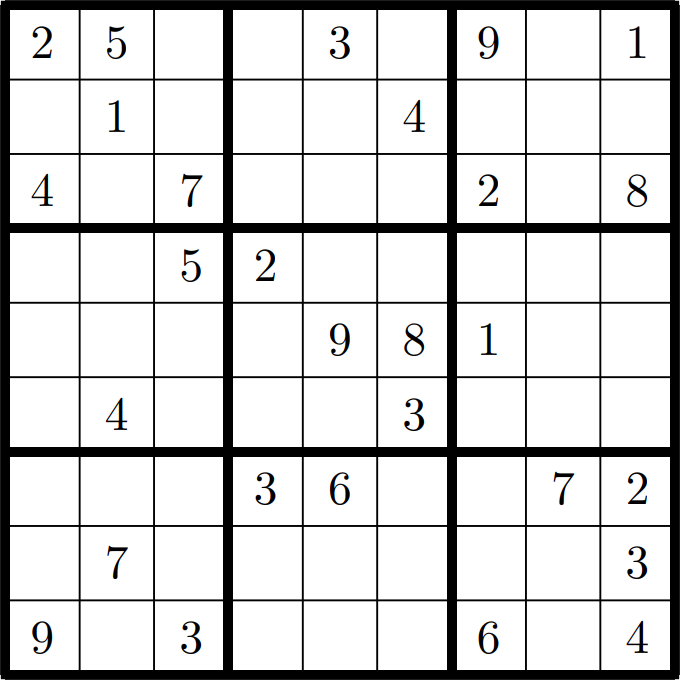
\includegraphics[width=0.5\linewidth]{figures/tut1-fig1.png}
            \caption*{Figure 1: A simple Sudoku puzzle.}
        \end{subfigure}
        \begin{subfigure}[t]{0.45\linewidth}
            \centering
            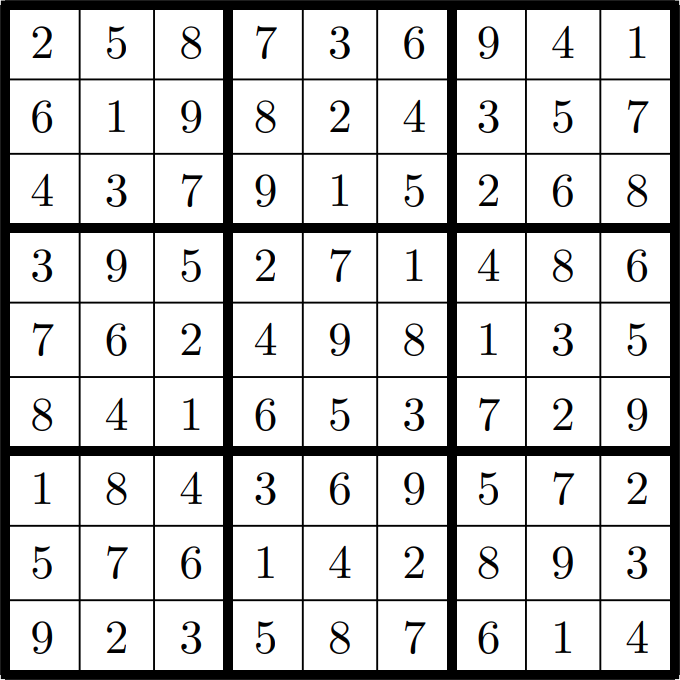
\includegraphics[width=0.5\linewidth]{figures/tut1-fig2.png}
            \caption*{Figure 2: Solution to the puzzle in Figure 1.}
        \end{subfigure}
    \end{figure}

    Sudoku puzzles can be solved easily after being modelled as a CSP (which will be covered later in the course). We will consider the problem of generating Sudoku puzzles. In particular, consider the following procedure: start with a completely full number grid (see Figure 2), and iteratively make some squares blank. We continue blanking out squares as long as the resulting puzzle can be completed in at least one way.

    Complete the following:

    \begin{listu}
        \item Give the representation of a state in this problem.

        \begin{solution}
            A state in this problem is a (partial) valid solution of the Sudoku puzzle. More formally, it would be a matrix $M \in \{ 0, \dots , 9 \}^{9\times9}$, with $0$ representing a blank square.
        \end{solution}

        \item Using the state representation defined above, specify the initial state and goal state(s).

        \begin{solution}
            \null

            \begin{listu}
                \item The initial state is a completed filled out grid of numbers which is a valid. All rows, columns, and $3 \times 3$ squares should contain all numbers between $1, \dots, 9$.
                \item Any state in the problem will be a valid goal state.
            \end{listu}
        \end{solution}

        \item Define its actions.

        \begin{solution}
            An action would be removing a number from the grid. More formally, we take as input a matrix $M$ and a matrix $E_{i,j}(a)$, where $E_{i,j}(a) \in \{ 0, \dots, 9 \}^{9 \times 9}$ is a matrix of all zeros except for a non-zero value $a \in \{ 1, \dots, 9 \}$ in coordinate $(i, j)$. An action would be setting $M - E_{i,j}(a)$.
        \end{solution}

        \item Using the state representation and actions defined above, specify the transition function $T$. (In other words, when each of the actions defined above is applied to a current state, what is the resulting state?)

        \begin{solution}
            The transition model would be $T(M - E_{ij}(a)) = M - E_{ij}(a)$.
        \end{solution}
    \end{listu}

    \item Assuming that ties (when pushing to the frontier) are broken based on alphabetical order, specify the order of the nodes that would be explored by the following algorithms. Assume that $S$ is the initial node, while $G$ is the goal node. You should express your answer in the form $S - B - A - F - G$ (i.e. no spaces, all uppercase letters, delimited by the dash ($-$) character), which, for example, corresponds to the exploration order of $S, B, A, F$, then $G$.

    \begin{figure}[ht!]
        \centering

        \tikzexternalenable
        \begin{tikzpicture} [every node/.style = {draw=black, circle}]

            \node (S) at (0,  0) {$S$};
            \node (A) at (2,  2) {$A$};
            \node (B) at (2,  0) {$B$};
            \node (C) at (2, -2) {$C$};
            \node (D) at (4,  0) {$D$};
            \node (E) at (4, -2) {$E$};
            \node (F) at (4,  2) {$F$};
            \node (G) at (6,  0) {$G$};

            \draw[thick,-latex] (S) -- (B);
            \draw[thick,-latex] (S) -- (C);
            \draw[thick,-latex] (A) -- (F);
            \draw[thick,-latex] (B) -- (A);
            \draw[thick,-latex] (B) -- (D);
            \draw[thick,-latex] (B) -- (E);
            \draw[thick,-latex] (C) -- (E);
            \draw[thick,-latex] (E) -- (D);
            \draw[thick,-latex] (F) -- (G);
        \end{tikzpicture}
        \tikzexternaldisable

        \caption*{Figure 3: Graph for question 2.}
    \end{figure}

    \begin{enumerate}
        \item Depth-First Search with no cycle-checking (aka tree-based) implementation.

        \begin{solution}
            $S - C - E - D - B - E - D - A - F - G$
        \end{solution}

        \item Breadth-First Search with no cycle-checking (aka tree-based) implementation.

        \begin{solution}
            $S - B - C - A - D - E - F - G$
        \end{solution}

        \item Breadth-First Search with cycle-checking (aka graph-based) implementation.

        \begin{solution}
            $S - B - C - A - D - E - F - G$
        \end{solution}
    \end{enumerate}

    \item \begin{enumerate}
        \item The \textbf{Breadth-First Search} algorithm is complete if the state space has infinite depth but finite branching factor.

        Determine if the statement above is True or False, and provide a rationale.

        \begin{solution}
            This is \textbf{true}.

            This follows immediately from the definitions of Breadth-First Search and completeness. (Recall that a search algorithm is complete if whenever there is a path from the initial state to the goal, the algorithm will find it.)

            In particular, the existence of a path means that the goal exists in a finite depth, and therefore Breadth-First Search will eventually reach it, since having a finite branching factor implies that the algorithm would not get lost in infinite-breadth search at some level.
        \end{solution}

        \item The \textbf{Breadth-First Search} algorithm can be complete even if zero step costs are allowed.

        Determine if the statement above is True or False, and provide a rationale

        \begin{solution}
            This is \textbf{true}.

            As highlighted in the previous question, Breadth-First Search is complete as long as the state space has a finite branching factor. Note that Breadth-First Search (as well as Depth-First Search) does not take into account edge weights.
        \end{solution}

        \item Given that a goal exists within a finite search space, the \textbf{Breadth-First Search} algorithm is cost-optimal if all step costs from the initial state are non-decreasing in the depth of the search tree. That is, for any given level of the search tree, all step costs are greater than the step costs in the previous level.

        Determine if the statement above is True or False, and provide a rationale

        \begin{solution}
            This is \textbf{false}.

            We could have two goal nodes in the same level with different costs but with the same depth. For example, arbitrary tie-breaking (or breaking ties by alphabetical ordering) of the Breadth-First Search algorithm may result in $A$ reached before $B$.

            \begin{figure}[ht!]
                \centering

                \tikzexternalenable
                \begin{tikzpicture}
                    \node[draw, circle] (S) at (0,  0) {$S$};
                    \node[draw, circle] (A) at (1, -1) {$A$};
                    \node[draw, circle] (B) at (2,  1) {$B$};

                    \draw[thick,-latex] (S) -- (A) node[midway, below left] {$9$};
                    \draw[thick,-latex] (S) -- (B) node[midway, above left] {$1$};
                \end{tikzpicture}
                \tikzexternaldisable

                \caption*{\color{primary}Figure 4: A counter-example for question 3c.}
            \end{figure}
        \end{solution}
    \end{enumerate}

    \item Prove that the \textbf{Uniform Cost Search} algorithm is cost-optimal as long as each step cost exceeds some small positive constant $\epsilon$.

    \begin{solution}
        \begin{proof}
            WTS UCS is optimal as long as each step cost exceeds positive value $\epsilon$.

            Given that each step cost exceeds some small positive constant $\epsilon$, completeness may be assumed. Consequently:

            \begin{listu}
                \item Whenever UCS expands a node $n$, the optimal path to that node has been found. If this was not the case, there would have to be another frontier node $n'$ on the optimal path from the start node to $n$. By definition, $n'$ would have a lower value of $g$ than $n$, and thus would have been selected first.

                \item If step costs are non-negative, paths never get shorter as nodes are added.
            \end{listu}

            The above two points imply that UCS expands nodes in the order of their optimal path cost.
        \end{proof}
    \end{solution}
\end{enumerate}

\newpage
\section*{Tutorial 2}

\subsection*{UCS}

Consider the search problem of Figure 1. Execute UCS (without cycle-checking) starting from node $S$, and the goal node being $G$.

\begin{figure}[ht!]
    \centering

    \tikzexternalenable
    \begin{tikzpicture}
        \node[draw,circle] (S) at (0,  0) {$S$};
        \node[draw,circle] (P) at (1, -1) {$P$};
        \node[draw,circle] (D) at (2,  2) {$D$};
        \node[draw,circle] (E) at (4,  2) {$E$};
        \node[draw,circle] (H) at (4,  0) {$H$};
        \node[draw,circle] (Q) at (3, -1) {$Q$};
        \node[draw,circle] (G) at (6,  0) {$G$};

        \draw[thick,-latex] (S) -- (D) node[midway, above left] {$3$};
        \draw[thick,-latex] (S) -- (P) node[midway, below left] {$1$};
        \draw[thick,-latex] (S) -- (E) node[midway, below     ] {$9$};
        \draw[thick,-latex] (P) -- (Q) node[midway, below     ] {$15$};
        \draw[thick,-latex] (D) -- (E) node[midway, above     ] {$2$};
        \draw[thick,-latex] (E) -- (H) node[midway,       left] {$1$};
        \draw[thick,-latex] (H) -- (Q) node[midway, above left] {$4$};
        \draw[thick,-latex] (Q) -- (G) node[midway, below     ] {$1$};
    \end{tikzpicture}
    \tikzexternaldisable

    \caption*{Figure 1: A search problem.}
\end{figure}

\begin{solution} \begin{table}[ht!] \color{primary}
    \centering
    \renewcommand{\arraystretch}{1.15}

    \begin{tabular}{r | l}
        (Node, Path)  & Frontier                                   \\ \hline
                      & $\{ (S, 0) \}$                             \\
        $(S, S)$      & $\{ (SP, 1), (SD, 3), (SE, 9) \}$          \\
        $(P, SP)$     & $\{ (SD, 3), (SE, 9), (SPQ, 16) \}$        \\
        $(D, SD)$     & $\{ (SDE, 5), (SE, 9), (SPQ, 16) \}$       \\
        $(E, SDE)$    & $\{ (SDEH, 6), (SE, 9), (SPQ, 16) \}$      \\
        $(H, SDEH)$   & $\{ (SE, 9), (SDEHQ, 10), (SPQ, 16) \}$    \\
        $(E, SE)$     & $\{ (SEH, 10), (SDEHQ, 10), (SPQ, 16) \}$  \\
        $(H, SEH)$    & $\{ (SDEHQ, 10), (SEHQ, 14), (SPQ, 16) \}$ \\
        $(Q, SDEHQ)$  & $\{ (DEHQG, 11), (SEHQ, 14), (SPQ, 16) \}$ \\
        $(G, SDEHQG)$ & $\{ (SEHQ, 14), (SPQ, 16) \}$              \\
    \end{tabular}
\end{table} \end{solution}

\subsection*{A* \& Heuristics}

A tracing example of executing A* (without cycle-checking) on the problem of figure 2

\begin{figure}[ht!]
    \centering

    \tikzexternalenable
    \begin{tikzpicture}
        \node[draw,circle] (A) at (0,   0) {$A$};
        \node[draw,circle] (B) at (0,  -2) {$B$};
        \node[draw,circle] (C) at (3,  -1) {$C$};
        \node[draw,circle] (D) at (3,  -3) {$D$};

        \draw[thick,-latex] (A)      -- (B)            node[midway,        left] {$4$};
        \draw[thick,-latex] (A)      -- (C)            node[midway, above      ] {$1$};
        \draw[thick,-latex] (B.east) -- (C.south west) node[midway, below      ] {$2$};
        \draw[thick,-latex] (C.west) -- (B.north east) node[midway, above      ] {$2$};
        \draw[thick,-latex] (B)      -- (D)            node[midway, below      ] {$6$};
        \draw[thick,-latex] (C)      -- (D)            node[midway,       right] {$9$};

        \node (hA) at (5,  0)   {$h(A) = 8$};
        \node (hB) at (5, -0.5) {$h(B) = 3$};
        \node (hC) at (5, -1)   {$h(C) = 7$};
        \node (hD) at (5, -1.5) {$h(D) = 0$};

        \node (start) at (5, -2.5) {START = $A$};
        \node (goal)  at (5, -3)   {GOAL = $D$};
    \end{tikzpicture}
    \tikzexternaldisable

    \caption*{Figure 2: Another search problem.}
\end{figure}

Each cost is depicted as the cost to get that node plus the heuristic cost at that node. Next node to be expanded is highlighted in blue. Here we maintain (Node, Path, Cost) as the tuple in the frontier.

\begin{table}[ht!]
    \centering
    \renewcommand{\arraystretch}{1.15}

    \begin{tabularx}{0.85\textwidth}{||c|Y||} % Adjust the table width and column width as needed
        \hline
        Node Popped & Frontier                                                                                                     \\ \hline \hline
                    & $\{ {\color{blue}(A,A, 0+8=8)} \}$                                                                           \\ \hline
        $A$         & $\{ (C,AC, 1+7=8), {\color{blue}(B,AB, 4+3=7)} \}$                                                           \\ \hline
        $B$         & $\{ {\color{blue}(C,AC, 1+7=8)}, (C,ABC, 6+7=13), (D,ABD, 10+0=10) \}$                                       \\ \hline
        $C$         & $\{ {\color{blue}(B,ACB, 3+3=6)}, (D,ACD, 10+0=10), (C,ABC, 6+7=13), (D,ABD, 10+0=10) \}$                    \\ \hline
        $B$         & $\{ (C,ACBC, 5+7=12), {\color{blue}(D,ACBD, 9+0=9)}, (D,ACD, 10+0=10), (C,ABC, 6+7=13), (D,ABD, 10+0=10) \}$ \\ \hline
    \end{tabularx}
\end{table}

\begin{enumerate}
    \item Execute A* with cycle-checking on the problem of figure 2.

    \begin{solution} \begin{table}[ht!] \color{primary}
        \centering
        \renewcommand{\arraystretch}{1.15}

        \begin{tabular}{||c|c||}
            \hline
            Node Popped & Frontier                                                \\ \hline \hline
                        & $\{ {\color{blue}(A,A, 0+8=8)} \}$                      \\ \hline
            $A$         & $\{ (C,AC, 1+7=8), {\color{blue}(B,AB, 4+3=7)} \}$      \\ \hline
            $B$         & $\{ {\color{blue}(C,AC, 1+7=8)}, (D,ABD, 10+0=10) \}$   \\ \hline
            $C$         & $\{ {\color{blue}(B,ACB, 3+3=6)}, (D,ABD, 10+0=10) \}$  \\ \hline
            $B$         & $\{ (C,ACBC, 5+7=12), {\color{blue}(D,ACBD, 9+0=9)} \}$ \\ \hline
        \end{tabular}
    \end{table} \end{solution}

    \item Prove that the A* Search algorithm with cycle-checking is optimal when a consistent heuristic is utilized.

    % TODO: Add solution

    \item In the search problem below, we have listed 5 heuristics. Indicate whether each heuristic is admissible and/or consistent in the table below.

    \begin{remark}
        \begin{listu}
            \item Consistent: $h(v_i) \le h(v_j) + c(v_i, v_j)$

            \item Admissible: $h(v) \le c^*(v)$
        \end{listu}
    \end{remark}

    \begin{table}[ht!]
        \centering

        \begin{tabular}{||c|c|c|c|c|c|c||}
            \hline
                  & S & A & B & G & Admissible            & Consistent            \\ \hline \hline
            $h_1$ & 0 & 0 & 0 & 0 & \color{primary} True  & \color{primary} True  \\ \hline
            $h_2$ & 8 & 1 & 1 & 0 & \color{primary} True  & \color{primary} False \\ \hline
            $h_3$ & 9 & 3 & 2 & 0 & \color{primary} True  & \color{primary} False \\ \hline
            $h_4$ & 6 & 3 & 1 & 0 & \color{primary} True  & \color{primary} True  \\ \hline
            $h_5$ & 8 & 4 & 2 & 0 & \color{primary} False & \color{primary} False \\ \hline
        \end{tabular}
    \end{table}

    \item Given that a heuristic $h$ is such that $h(s_g) = 0$ where $s_g$ is any goal state, prove that if $h$ is consistent, then it must be admissible

    % TODO: Add solution

    \item \begin{enumerate}[label=\alph*)]
        \item Provide a counter-example to show that the \textbf{Greedy Best-First Search} algorithm without cycle-checking is incomplete.

        \begin{solution}
            % \begin{center} \begin{tikzpicture}
            %     \node[draw,circle] (S0) at (0, 0) {$S_0$};
            % \end{tikzpicture} \end{center}
            % TODO: Add solution
        \end{solution}

        \item Provide a counter-example to show that Greedy Best-First Search (with or without cycle-checking) is not optimal.

        % TODO: Add solution
    \end{enumerate}
\end{enumerate}